\documentclass[UTF8,12pt]{ctexart}
\ctexset{section={name={},number=\chinese{section}}}
\usepackage{fontspec}
\usepackage{xeCJK}
\usepackage{abstract}
\usepackage{geometry}
\usepackage{amsmath}
\numberwithin{equation}{section}%公式按章节编号
\usepackage{graphicx}
\usepackage{subfigure}
\usepackage{indentfirst}
\usepackage{setspace}
\usepackage{newproof}
\usepackage{bm}%加粗公式的包,在需要加粗的公式前面加\bm
%以下代码以及listings包为添加有中文注释的latex代码的模块
\usepackage{listings}
  \usepackage{xcolor}
  \lstset{tabsize=4, %
  frame=shadowbox, %把代码用带有阴影的框圈起来
  commentstyle=\color{red!50!green!50!blue!50},%浅灰色的注释
  rulesepcolor=\color{red!20!green!20!blue!20},%代码块边框为淡青色
  keywordstyle=\color{blue!90}\bfseries, %代码关键字的颜色为蓝色,粗体
  showstringspaces=false,%不显示代码字符串中间的空格标记
  stringstyle=\ttfamily, % 代码字符串的特殊格式
  keepspaces=true, %
  breakindent=22pt, %
  numbers=left,%左侧显示行号
  stepnumber=1,%
  numberstyle=\tiny, %行号字体用小号
  basicstyle=\footnotesize, %
  showspaces=false, %
  flexiblecolumns=true, %
  breaklines=true, %对过长的代码自动换行
  breakautoindent=true,%
  breakindent=4em, %
  escapebegin=\begin{CJK*}{GBK}{hei},escapeend=\end{CJK*},
  aboveskip=1em, %代码块边框
  fontadjust,
  captionpos=t,
  framextopmargin=2pt,framexbottommargin=2pt,abovecaptionskip=-3pt,belowcaptionskip=3pt,
  xleftmargin=4em,xrightmargin=4em, % 设定listing左右的空白
  texcl=true,
  % 设定中文冲突,断行,列模式,数学环境输入,listing数字的样式
  extendedchars=false,columns=flexible,mathescape=true
  % numbersep=-1em
}
\usepackage{algorithm}
\usepackage{algpseudocode}
\usepackage{amsmath}
\usepackage{hyperref}%ref引用,可以定义不同引用的颜色
\hypersetup{colorlinks=true,
            linkcolor=black,
            anchorcolor=blue,
            citecolor=blue}
\usepackage[natbibapa,nodoi]{apacite}

%% 写算法伪代码或者流程的前期准备
\renewcommand{\algorithmicrequire}{\textbf{Input:}}  % Use Input in the format of Algorithm
\renewcommand{\algorithmicensure}{\textbf{Output:}} % Use Output in the format of Algorithm
\renewcommand{\contentsname}{\hspace*{\fill}目\quad 录\hspace*{\fill}}
%跨页伪代码↓
\usepackage{algpseudocode} 
\makeatletter
\newenvironment{breakablealgorithm}
  {% \begin{breakablealgorithm}
   \begin{center}
     \refstepcounter{algorithm}% New algorithm
     \hrule height.8pt depth0pt \kern2pt% \@fs@pre for \@fs@ruled
     \renewcommand{\caption}[2][\relax]{% Make a new \caption
       {\raggedright\textbf{\ALG@name~\thealgorithm} ##2\par}%
       \ifx\relax##1\relax % #1 is \relax
         \addcontentsline{loa}{algorithm}{\protect\numberline{\thealgorithm}##2}%
       \else % #1 is not \relax
         \addcontentsline{loa}{algorithm}{\protect\numberline{\thealgorithm}##1}%
       \fi
       \kern2pt\hrule\kern2pt
     }
  }{% \end{breakablealgorithm}
     \kern2pt\hrule\relax% \@fs@post for \@fs@ruled
   \end{center}
  }
\makeatother

\newtheorem{Definition}{\hspace{2em}定义}
\newtheorem{theorem}{\hspace{2em}定理}
\newtheorem{lemma}{\hspace{2em}引理}
\newtheorem{Proof}{\hspace{2em}证明}%*意为去掉编号
\newtheorem{example}{\hspace{2em}例}
%用于自动替换中文标点为英文符号
\catcode`\。=\active
\newcommand{。}{. }
\catcode`\,=\active
\newcommand{,}{, }

\setlength{\parindent}{2em}%首行缩进
\lstset{extendedchars=false}%解决代码跨页时,章节标题,页眉等汉字不显示的问题

\geometry{left=3.0cm,right=3.0cm,top=2.54cm,bottom=2.54cm}
\title{{\heiti\fontsize{40}{15}\selectfont 最优化方法上级报告}\\[1em]
\fontsize{25}{15}\selectfont \textbf{}\\[7em]}
\author{\fontsize{20}{20}\selectfont \textit{信计}91 \quad \textit{闻逊之}\\[1em]
\fontsize{20}{20}\selectfont \textit{学号}:2193410365\\[2.5em]}
\date{\Large\today\\[1em]\Large {(2021-2022春季学期)}}
\linespread{1.2}
\pagestyle{plain}

\begin{document}
    \begin{figure}[t]
    \parbox[b]{2cm}{
        
\includegraphics[scale=0.3]{D:/Adam_Wen/CoverSet/红色校徽校标.png}
        }
\end{figure}
    
    \maketitle
    \newpage


    \newpage
    \section{作业4第一题}
    \subsection{题目阐述}
    分别用0.618法和三点二次插值法求$ \phi(\alpha) = 1-\alpha e^{-\alpha^2}  $的
    极小点,初始区间取$ [0,1] ,\epsilon = 0.001$.
    \subsection{绘制函数图像}
    $ \phi(\alpha) = 1-\alpha e^{-\alpha^2}  $的函数图像如图\ref{1_Func}所示,可见函数
    呈高-低-高形状,在目标区间内是单峰函数,满足0.618法以及三点二次插值法的应用条件。
    \par
    容易算出函数的理论极小点为$ \frac{\sqrt{2}}{2} $。 
    \begin{figure}[h!]
        \centering
        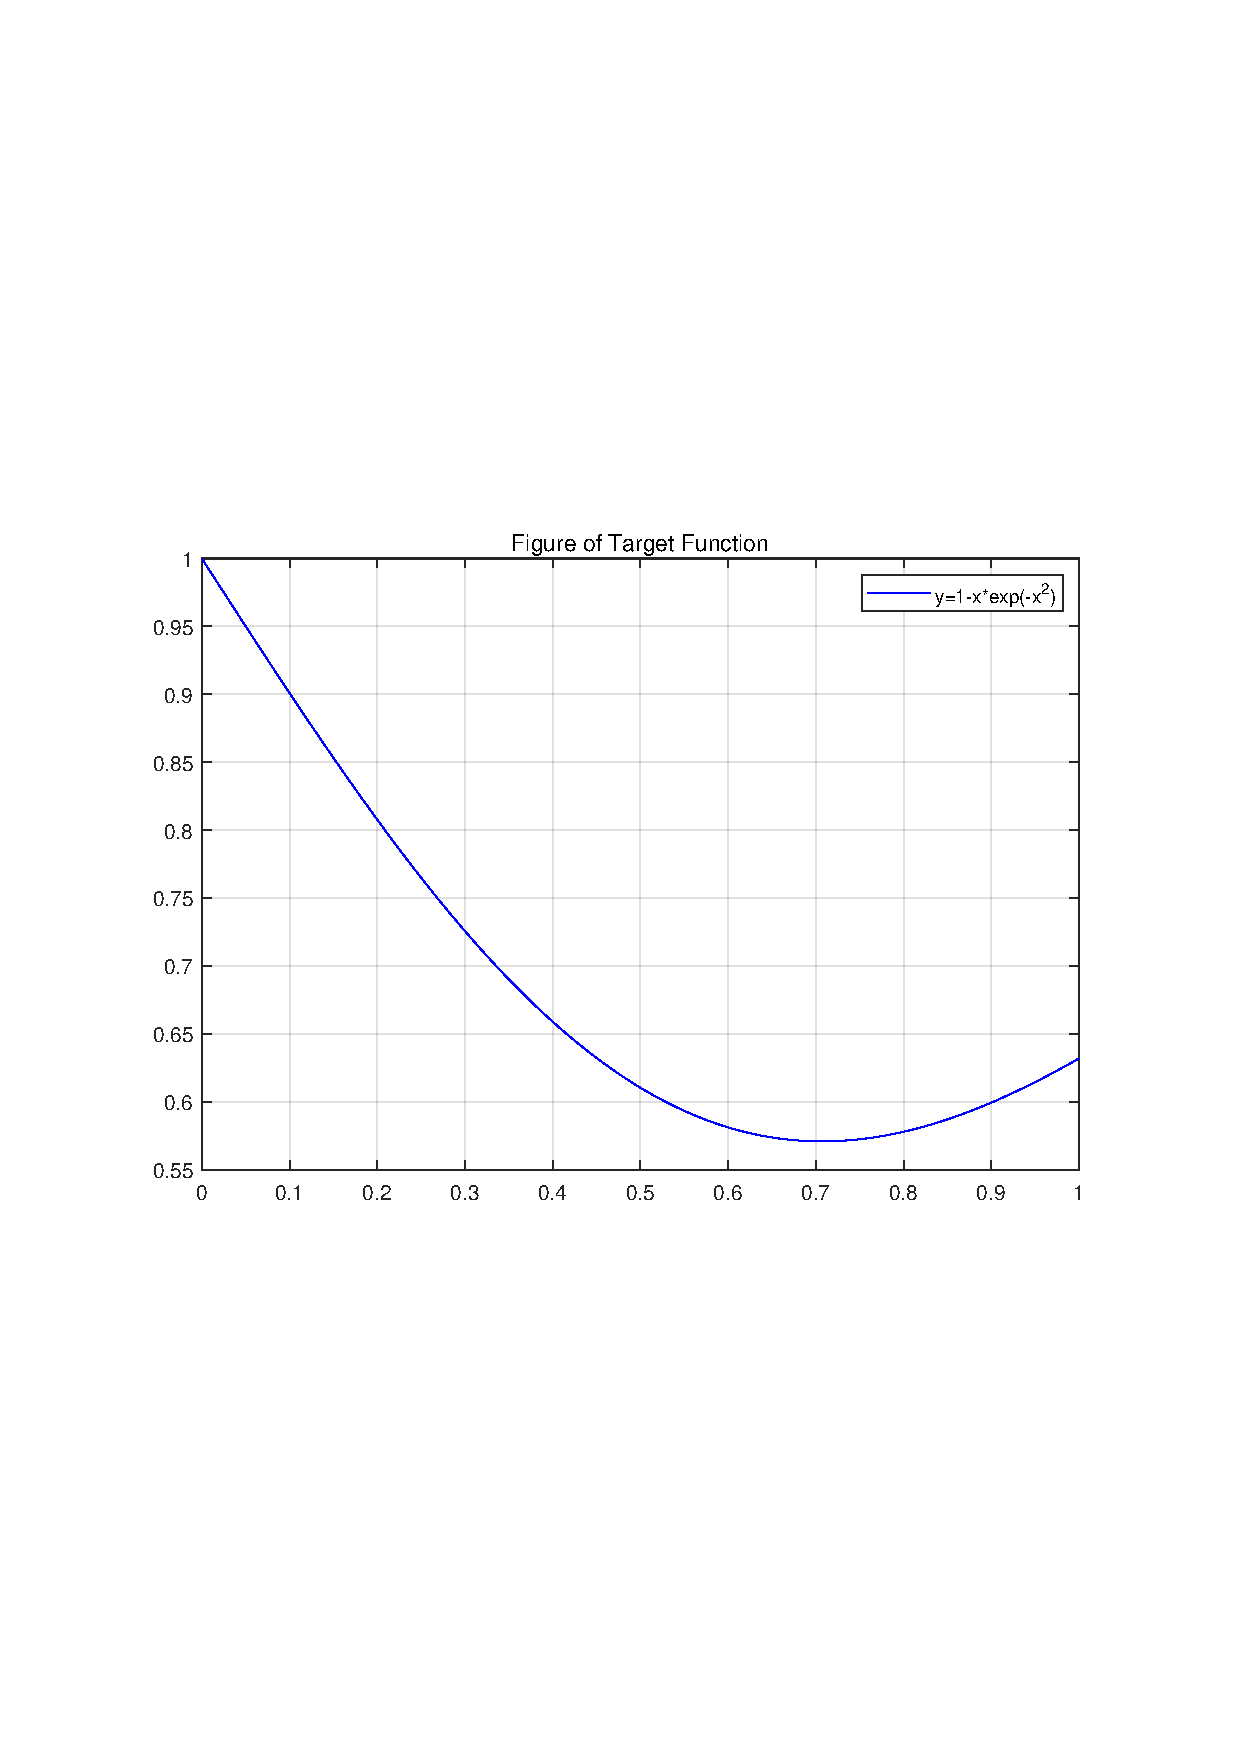
\includegraphics[width = 14cm]{第一题-Func.pdf}
        \caption[]{目标函数图像}\label{1_Func}
    \end{figure}
    \newpage
    \subsection{0.618法结果及程序}
    0.618法求得的结果为$ \alpha^*=0.7069965 $,其迭代次数与误差距离的图像如图\ref{1_0.618}
    所示.
    \begin{figure}[htbp!]
        \centering
        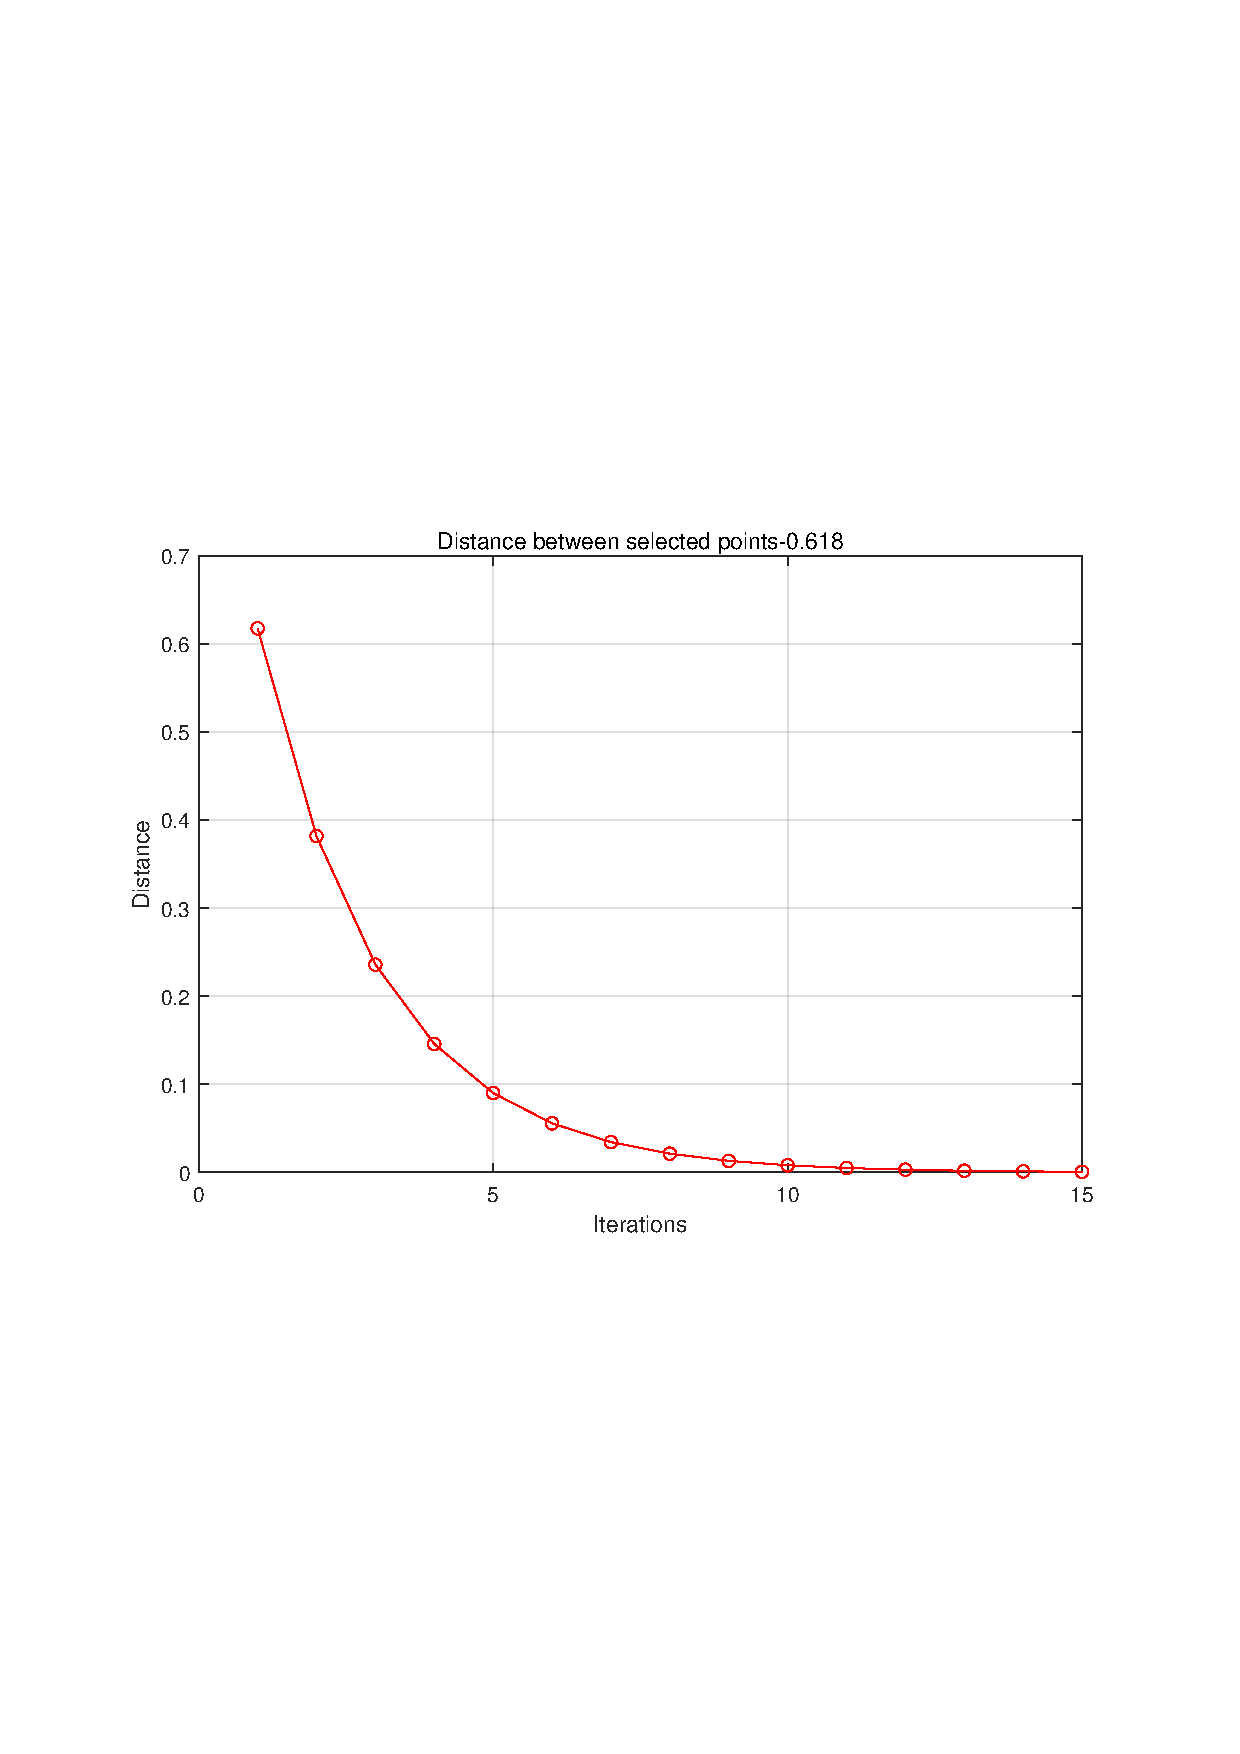
\includegraphics[width = 14cm]{第一题-0.618.pdf}
        \caption[]{0.618法误差收敛图像}\label{1_0.618}
    \end{figure} 

    \begin{center}
            \textbf{0.618法matlab代码}
    \end{center}

    \lstinputlisting[language=matlab]{FirstAssignment/func_618.m}

    \subsection{三点二次插值法结果及程序}
    三点二次插值法求得的结果为$ \alpha^*=0.69559476 $,其迭代次数与误差距离额图像如图\ref{1_3_2}所示

    \begin{figure}[htbp!]
        \centering
        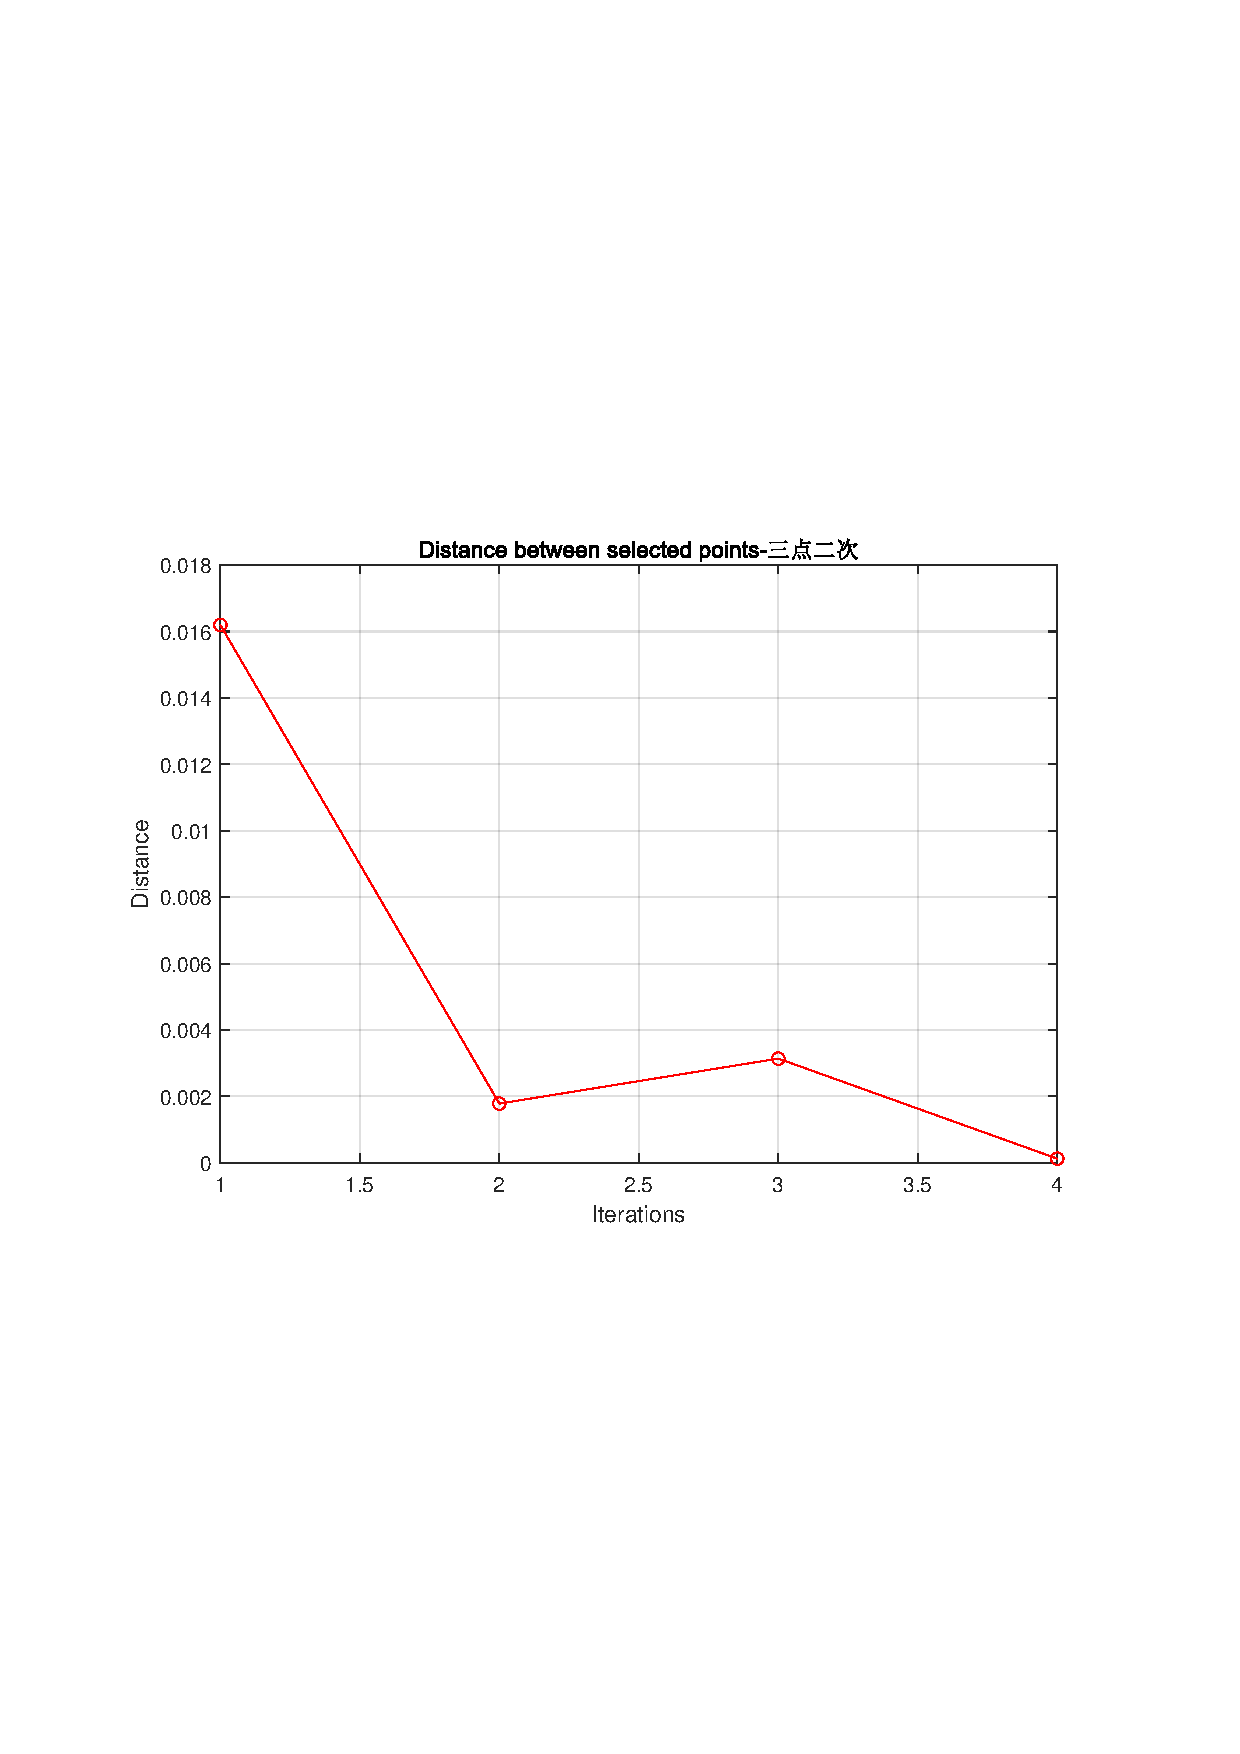
\includegraphics[width = 14cm]{第一题-三点二次.pdf}
        \caption[]{三点二次插值法误差收敛图像}\label{1_3_2}
    \end{figure} 

    \begin{center}
        \textbf{三点二次插值法matlab代码}
    \end{center}

    \lstinputlisting[language=matlab]{FirstAssignment/func_3_2.m}


    \section{作业7第三题}
    \subsection{题目阐述}
    编写SR1方法,DFP方法和BFGS方法程序并提供数值实验结果报告。考虑最优化问题:
    \[
        min\sum \limits_{i=1}^m r_i^2(\bm{x}) 
    \] 
    其中,$ r_i(\bm{x}) $由Watson函数定义:
    \[
        r_i(\bm{x}) = \sum \limits_{j=2}^n(j-1)x_jt_i^{j-2}-(\sum\limits_{j=1}^n 
        x_jt_i^{j-1} )^2-1  
    \]  
    其中$ t_i = \frac{i}{29} \quad 1\leq i\leq 29, r_{30}(\bm{x}) = x_1, r_{31} = x_2-x_1^2-1, 2\leq n
    \leq 31,m =31 $,初始值可选为$ x^{(0)} = (0,\cdots,0)^T  $  

    考虑到计算机性能等问题,下文展示$ n=2 $时的图像结果与$ n=3 $时的数值结果. 
    
    算法采用Armijo准则确定搜索步长,$ \rho = 0.001 $ .
    \subsection{SR1法}
    当$ n=2 $时,函数值的更新如图\ref{SR1-func}所示,其梯度数值的变化如图\ref{SR1-grad}所示:
    \par
    最终迭代次数为14次,极小点为$ (-0.50137,1.0736) $ ,函数值为$ 0.54661. $ 
    \begin{figure}[htbp!]
        \centering
        \subfigure[SR1法迭代路径]{
            \centering
            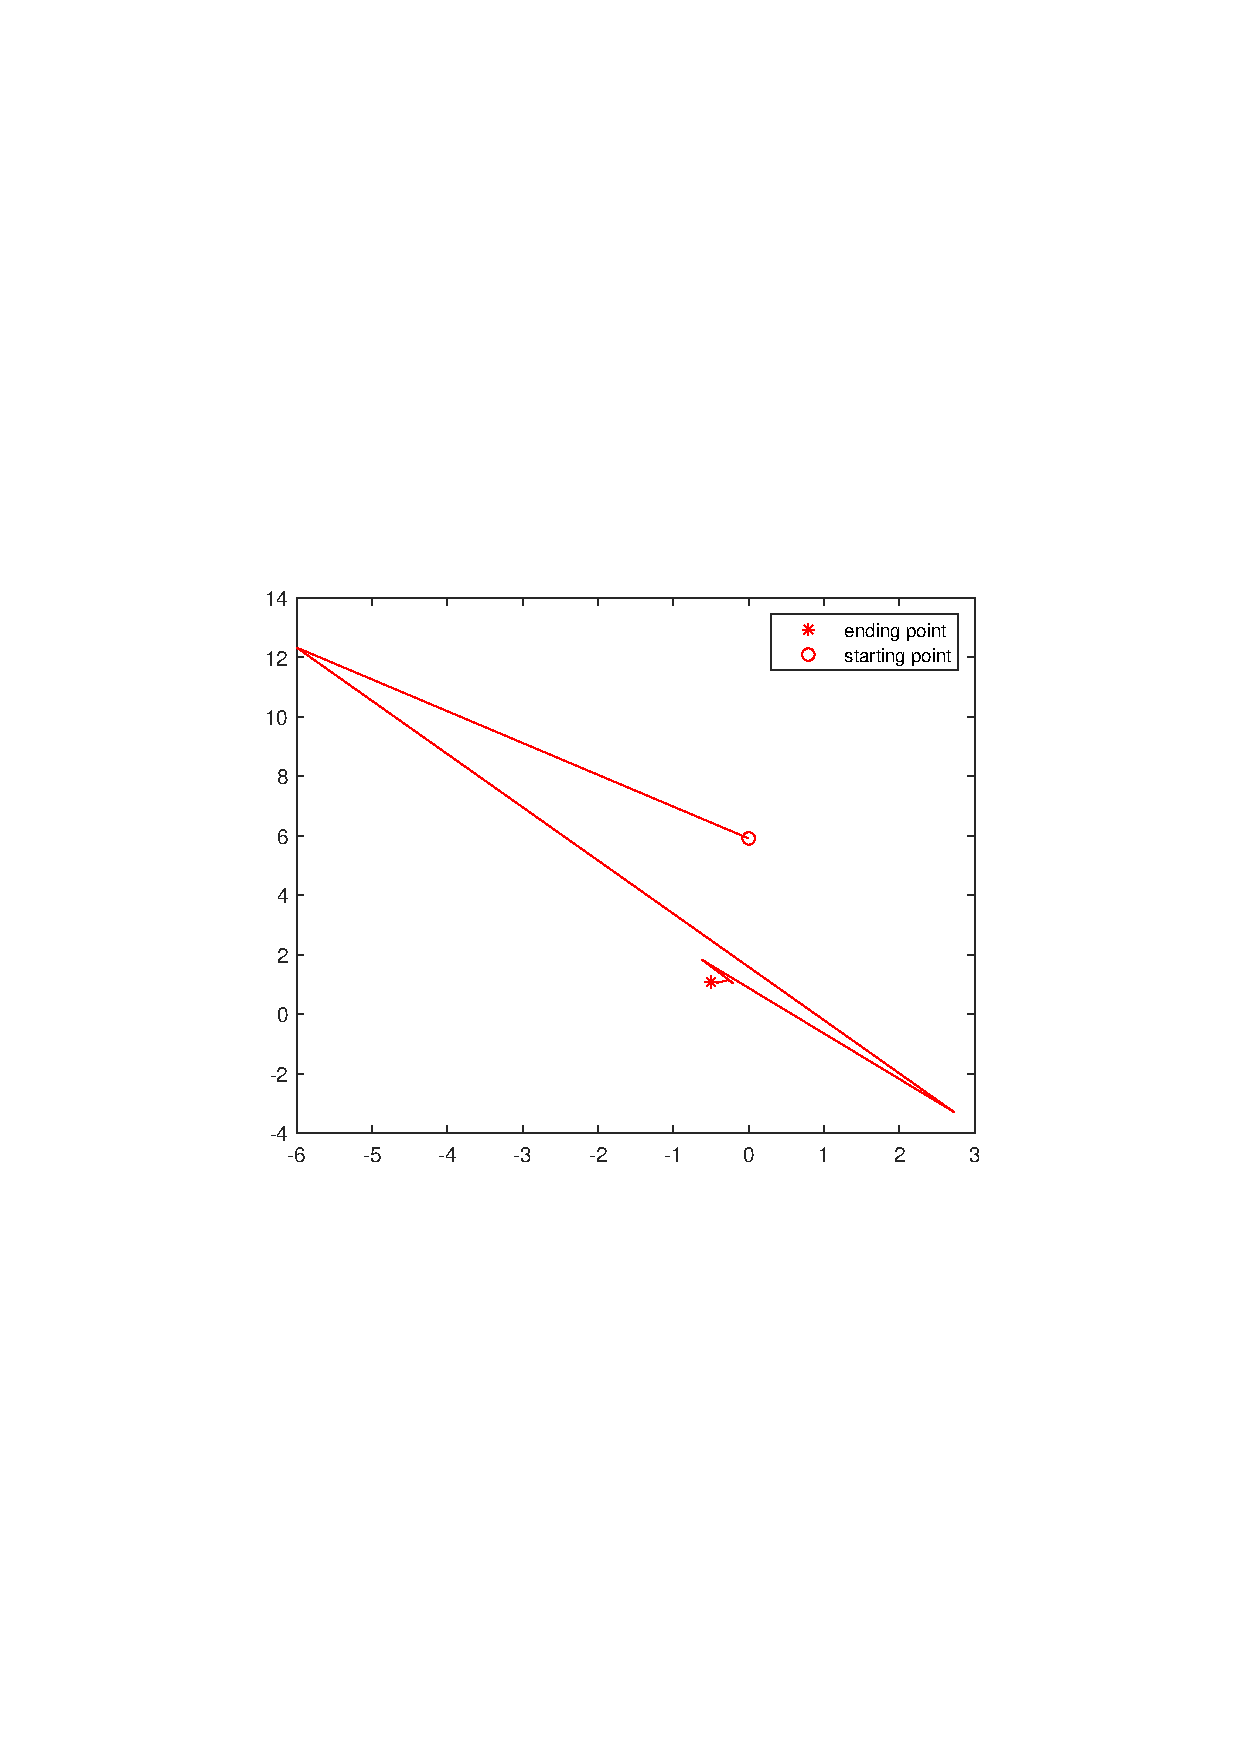
\includegraphics[width=7.5cm]{第二题-SR1-func.pdf}\label{SR1-func}}
            \subfigure[SR1法梯度数值变化]{
        \centering
        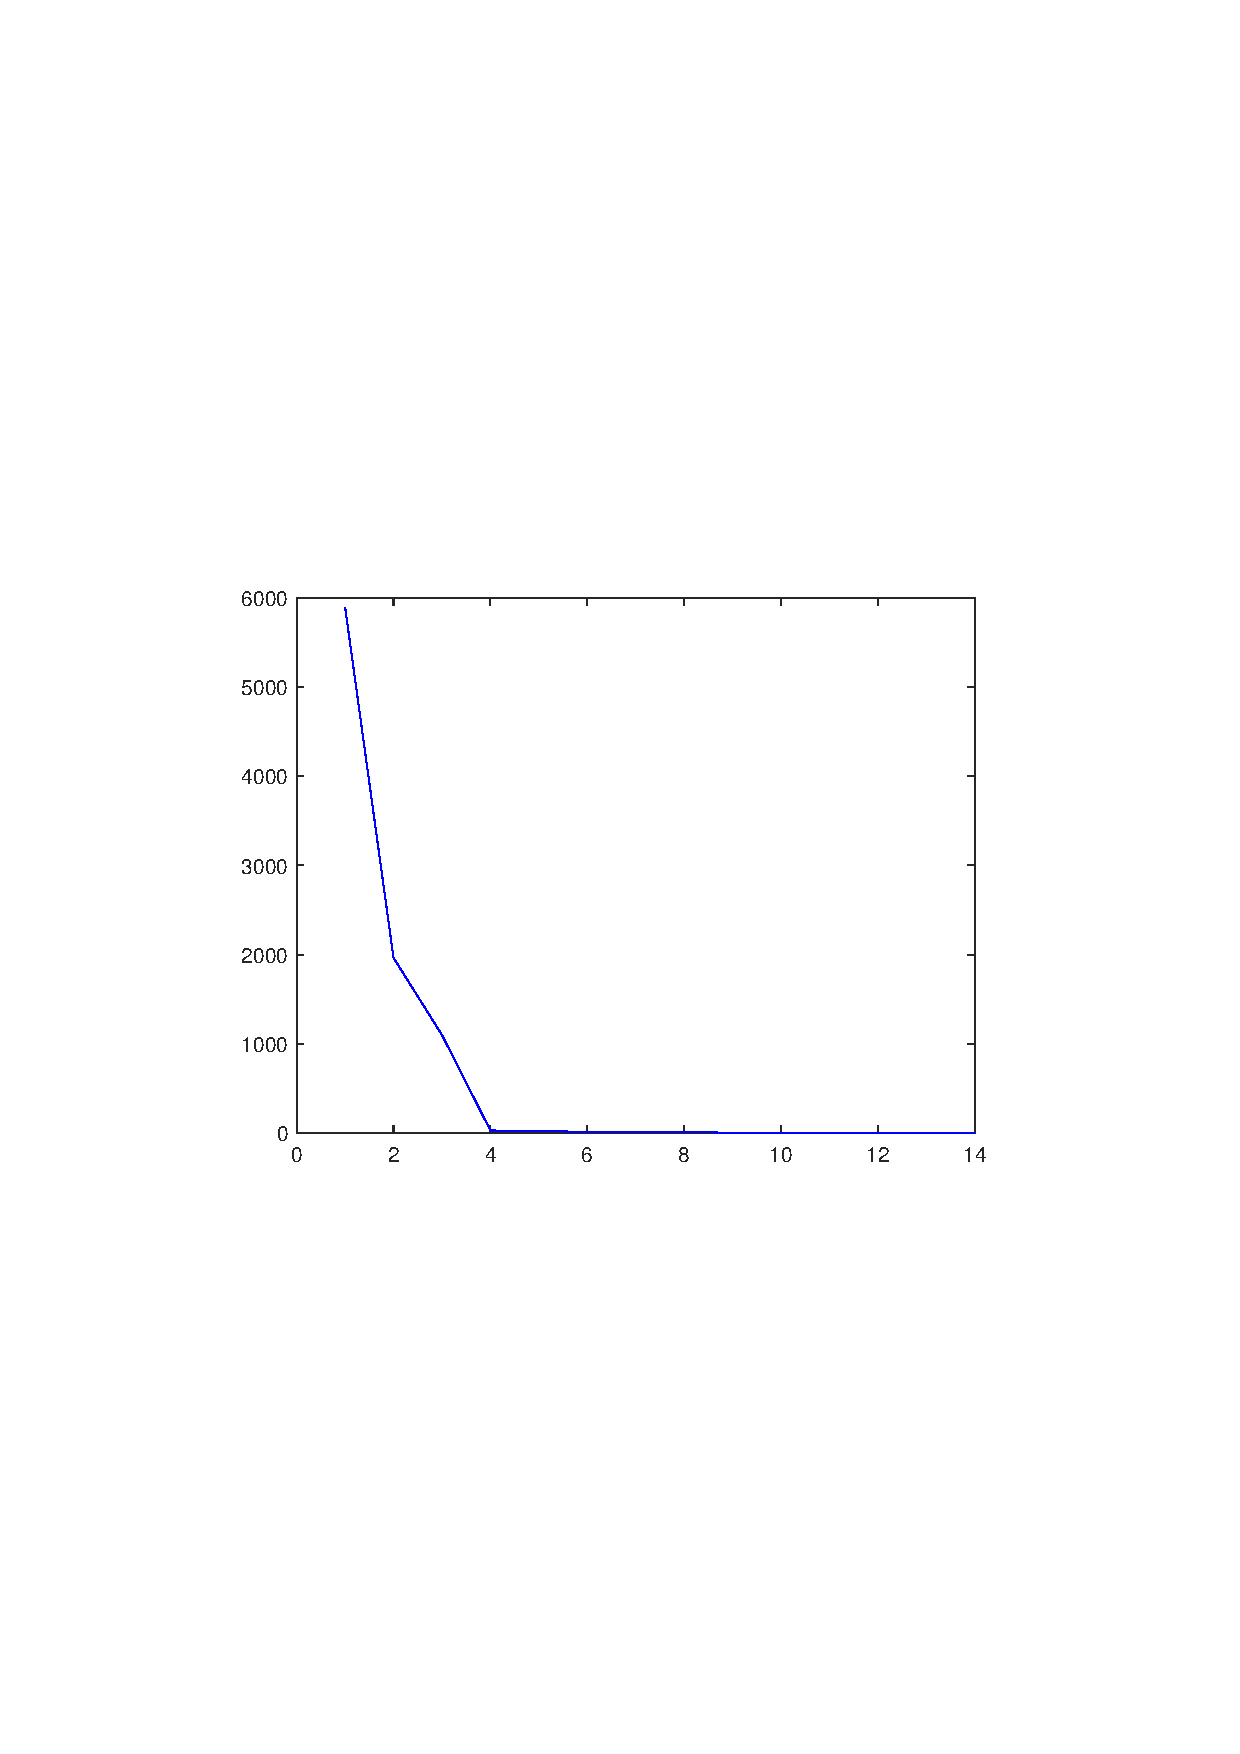
\includegraphics[width=7.5cm]{第二题-SR1-grad.pdf}\label{SR1-grad}}
        \caption{SR1法结果图,$ n=2 $ }
    \end{figure}

    当$ n=3 $时,最终迭代次数为$23$ 次,极小点为$ (-0.37573,0.92779,0.17164) $ ,函数值为$ 0.4714 $ .

    \subsection{DFP法}
    当$ n=2 $时,函数值的更新如图\ref{DFP-func}所示,其梯度数值的变化如图\ref{DFP-grad}所示:
    \par
    最终迭代次数为58次,极小点为$ (-0.50137,1.0736) $ ,函数值为$ 0.54661. $ 
    \begin{figure}[htbp!]
        \centering
        \subfigure[DFP法迭代路径]{
            \centering
            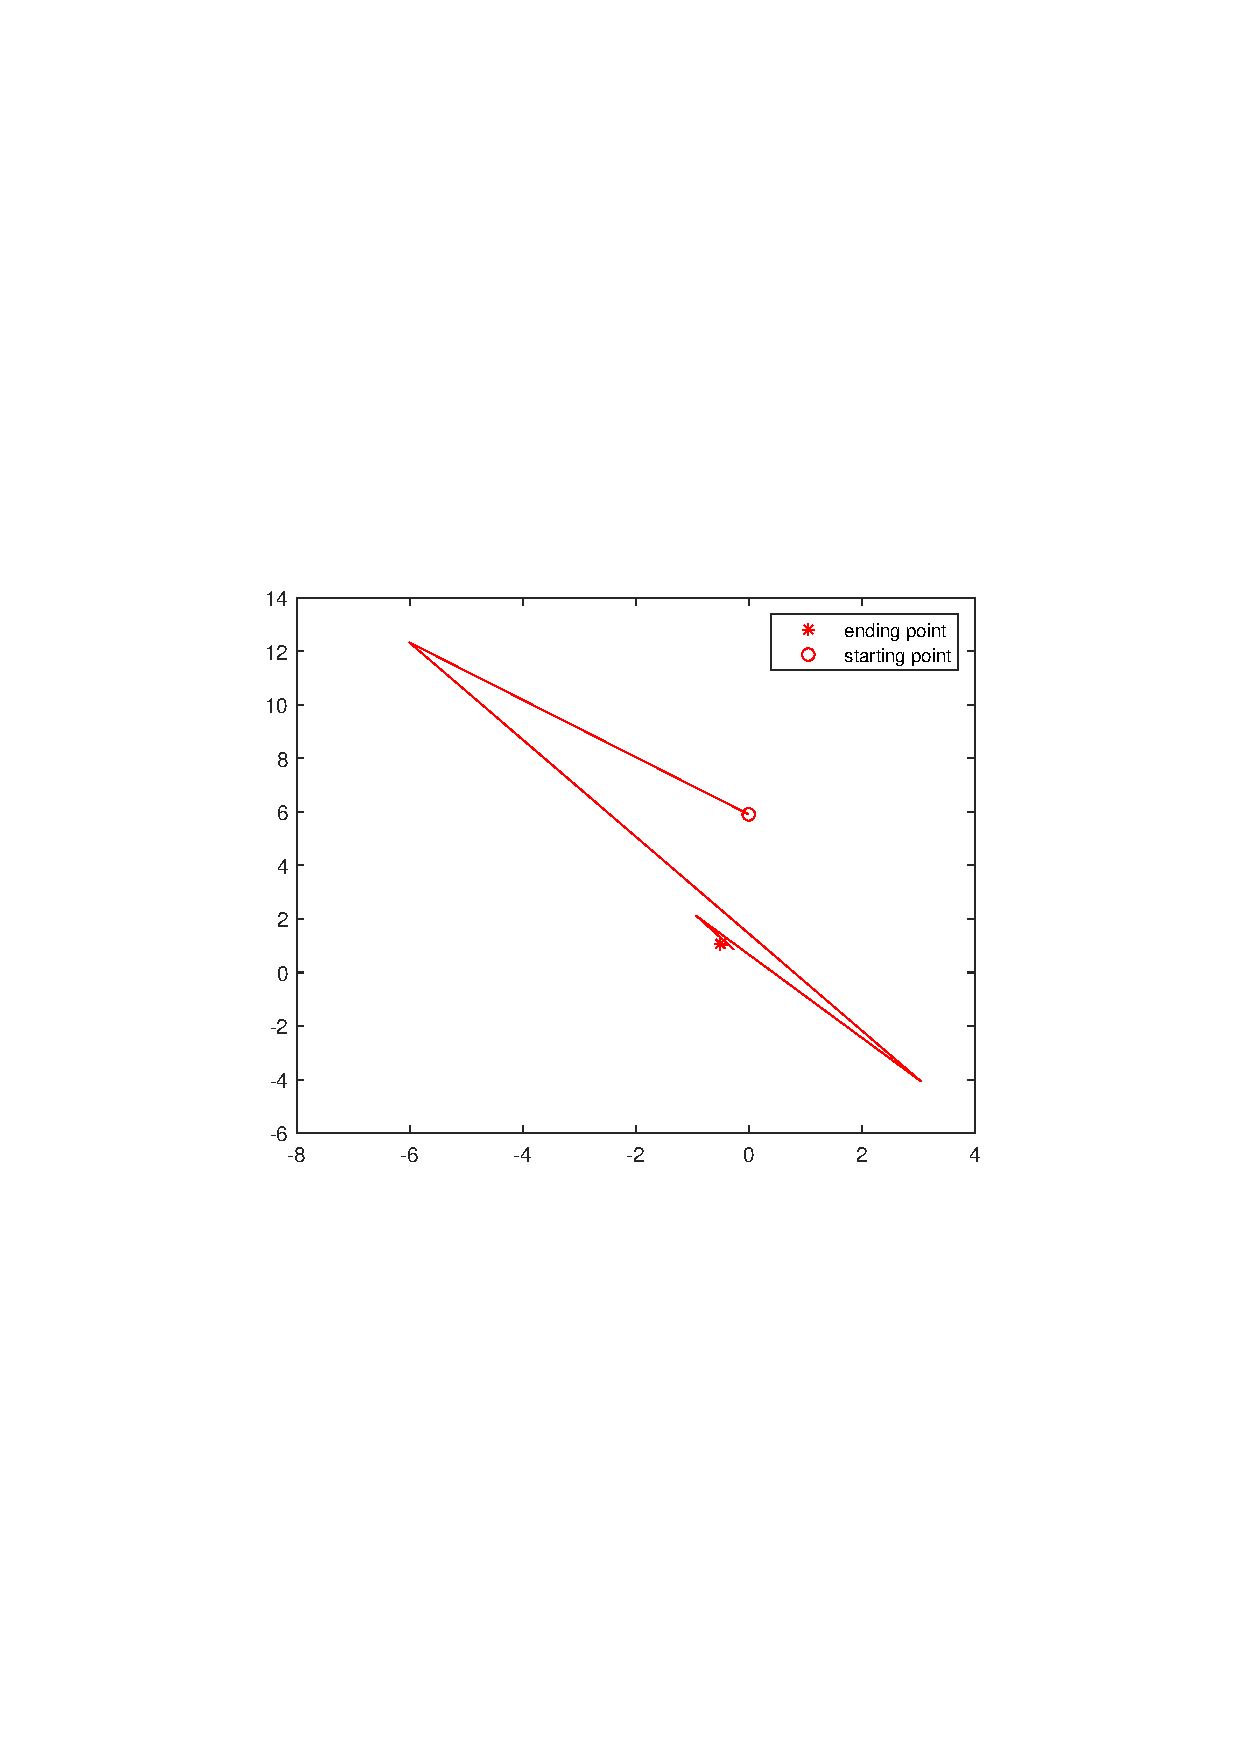
\includegraphics[width=7.5cm]{第二题-DFP-func.pdf}\label{DFP-func}}
            \subfigure[DFP法梯度数值变化]{
        \centering
        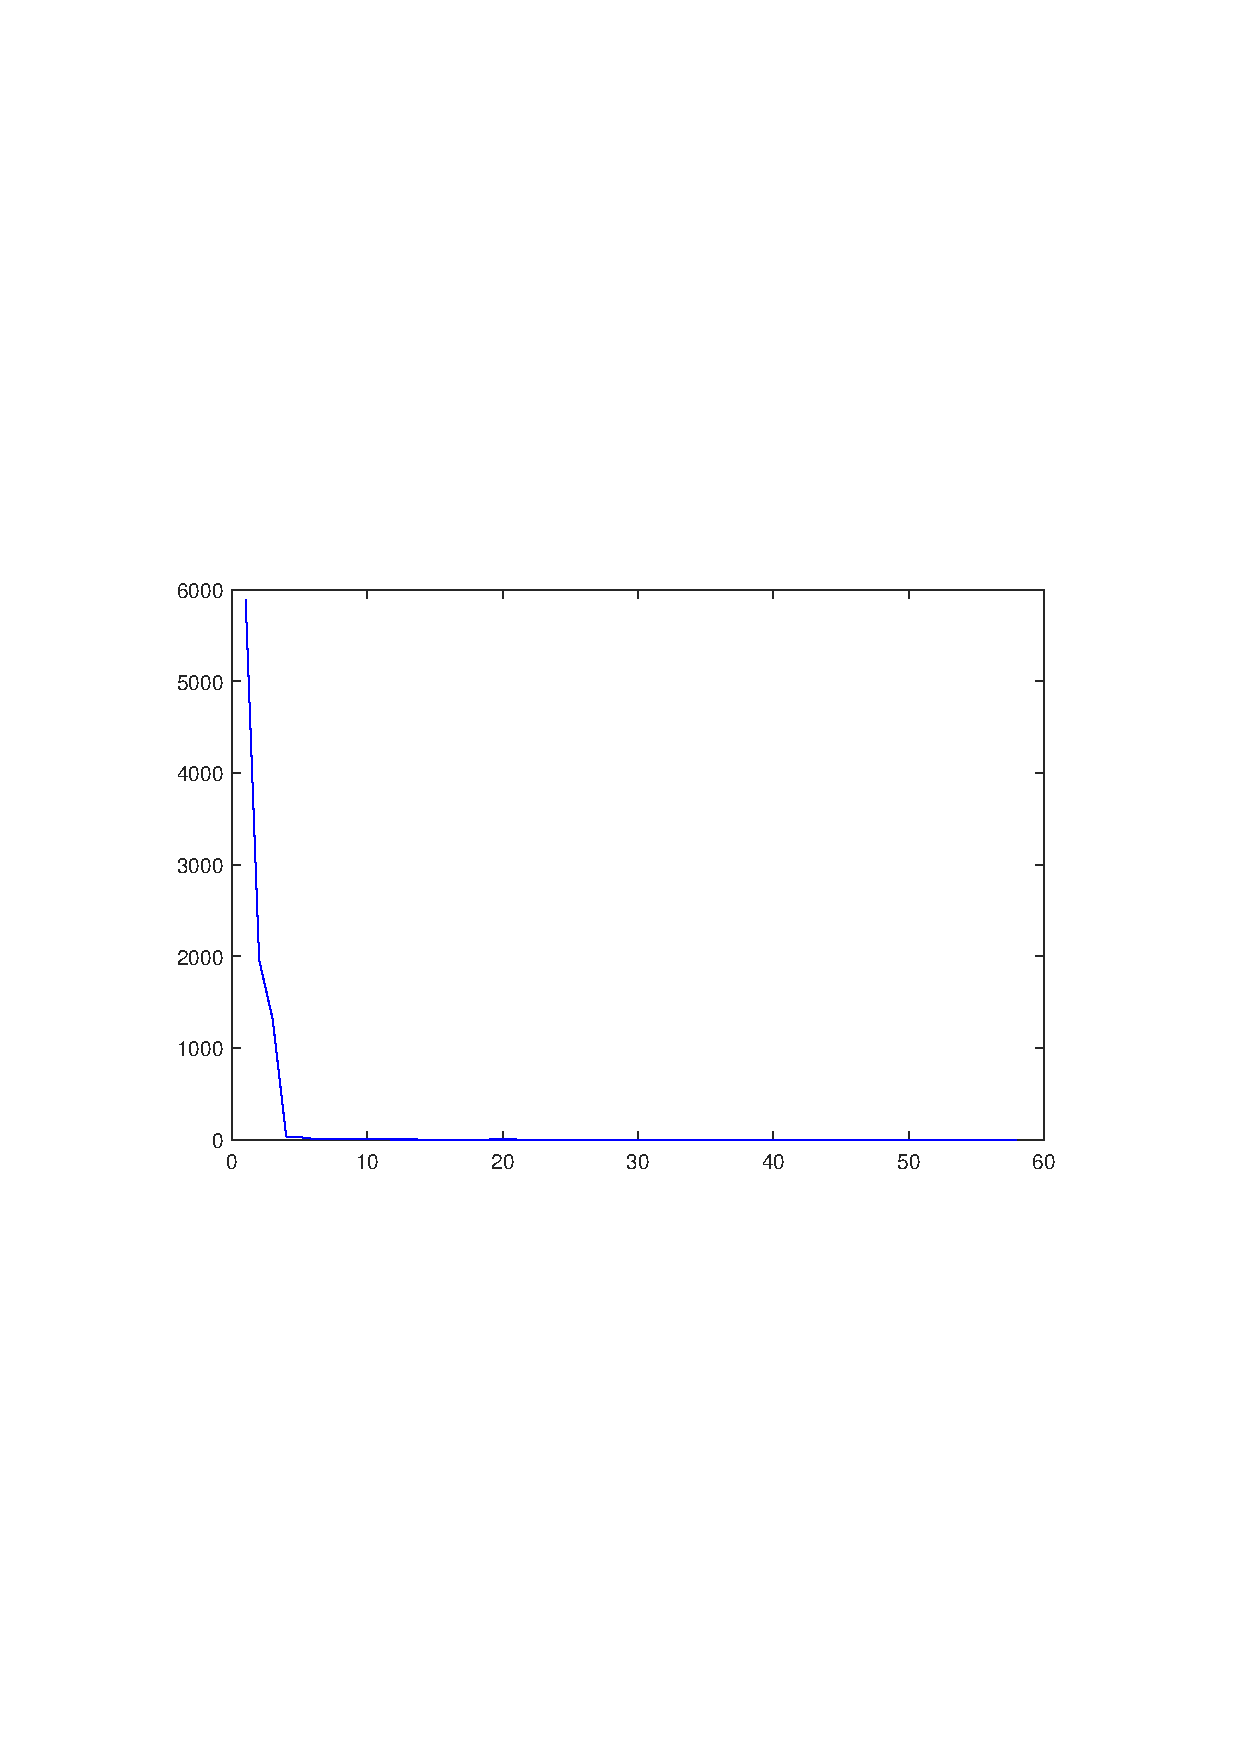
\includegraphics[width=7.5cm]{第二题-DFP-grad.pdf}\label{DFP-grad}}
        \caption{DFP法结果图,$ n=2 $ }
    \end{figure}

    当$ n=3 $时,最终迭代次数为$ 386 $ 次,极小点为$ (-0.37573,0.92779,0.17164) $ ,函数值为$ 0.4714 $ .

    \subsection{BGFS法}
    当$ n=2 $时,函数值的更新如图\ref{BFGS-func}所示,其梯度数值的变化如图\ref{BFGS-grad}所示:
    \par
    最终迭代次数为15次,极小点为$ (-0.50137,1.0736) $ ,函数值为$ 0.54661. $ 
    \begin{figure}[htbp!]
        \centering
        \subfigure[BFGS法迭代路径]{
            \centering
            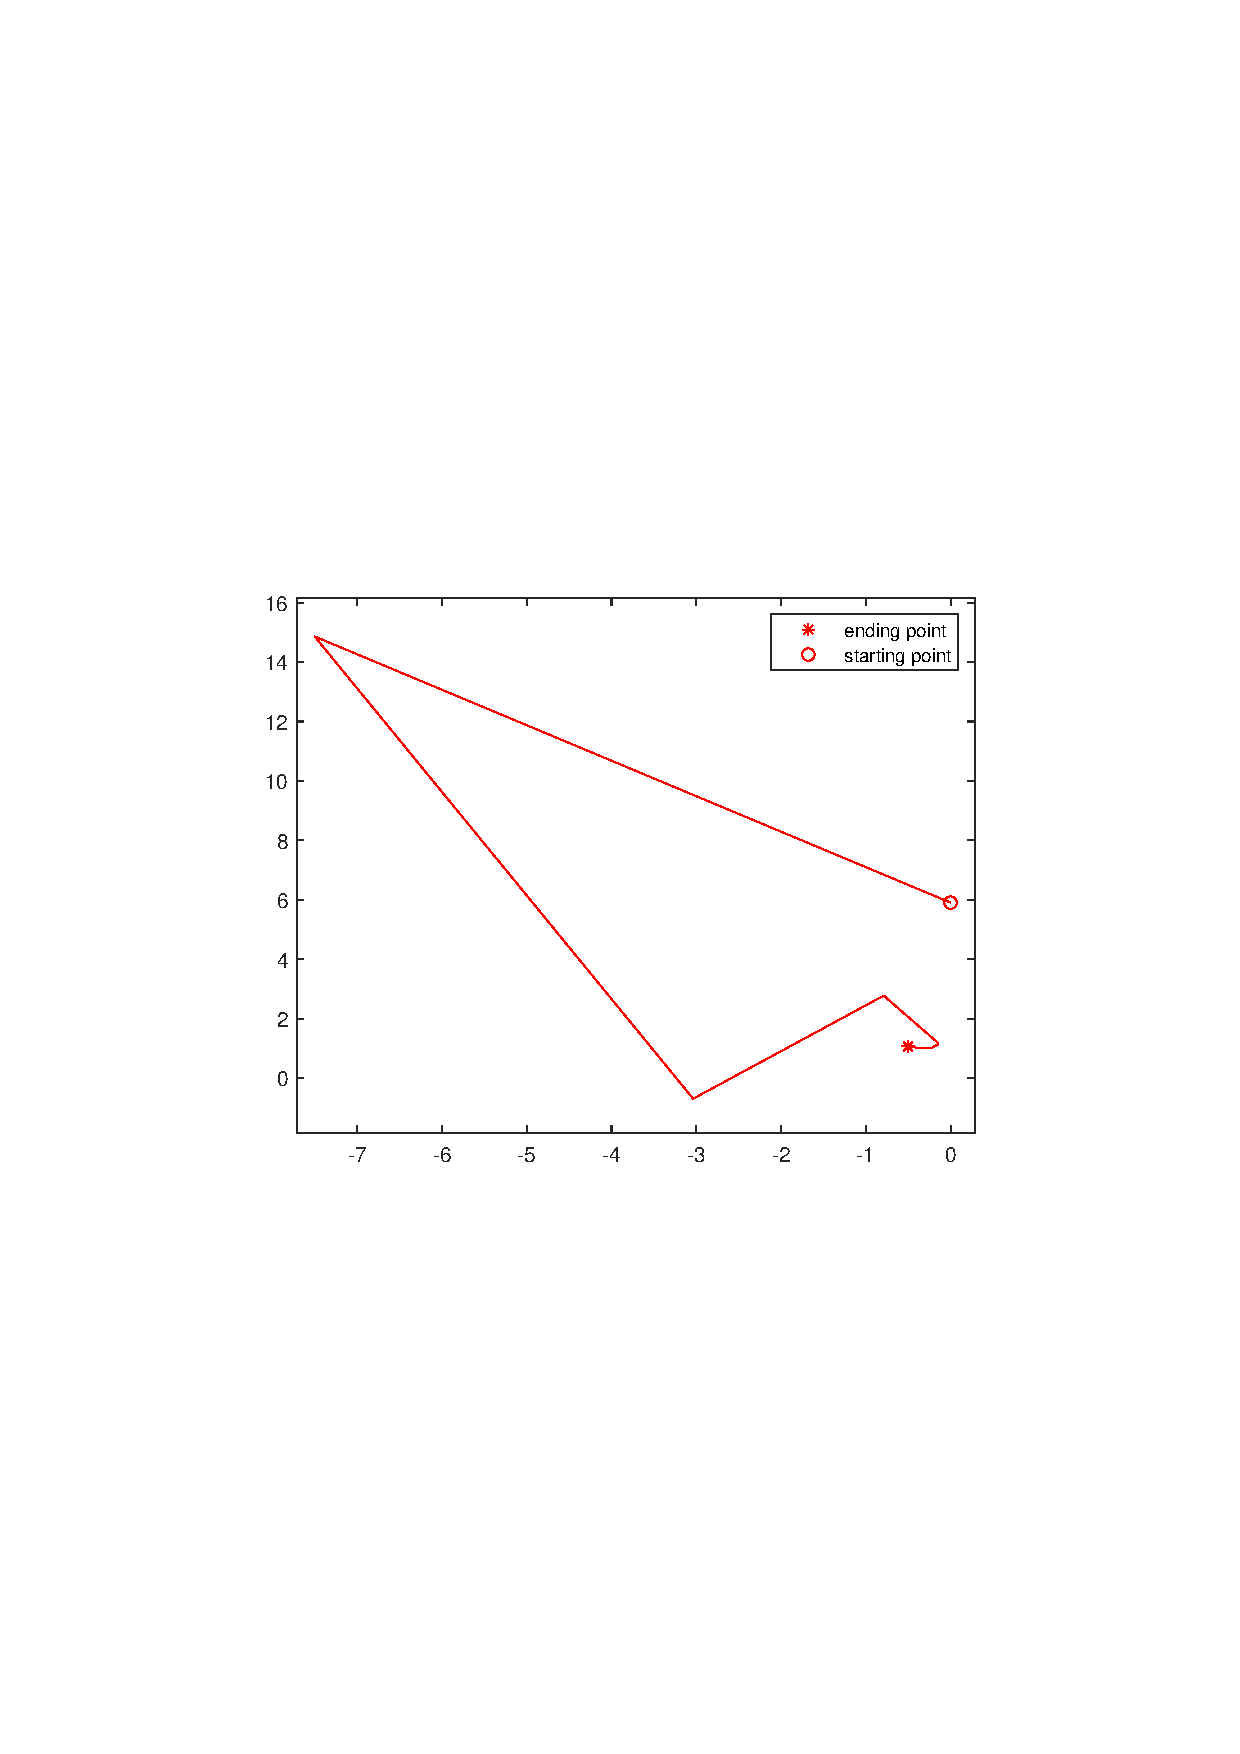
\includegraphics[width=7.5cm]{第二题-BFGS-func.pdf}\label{BFGS-func}}
            \subfigure[BFGS法梯度数值变化]{
        \centering
        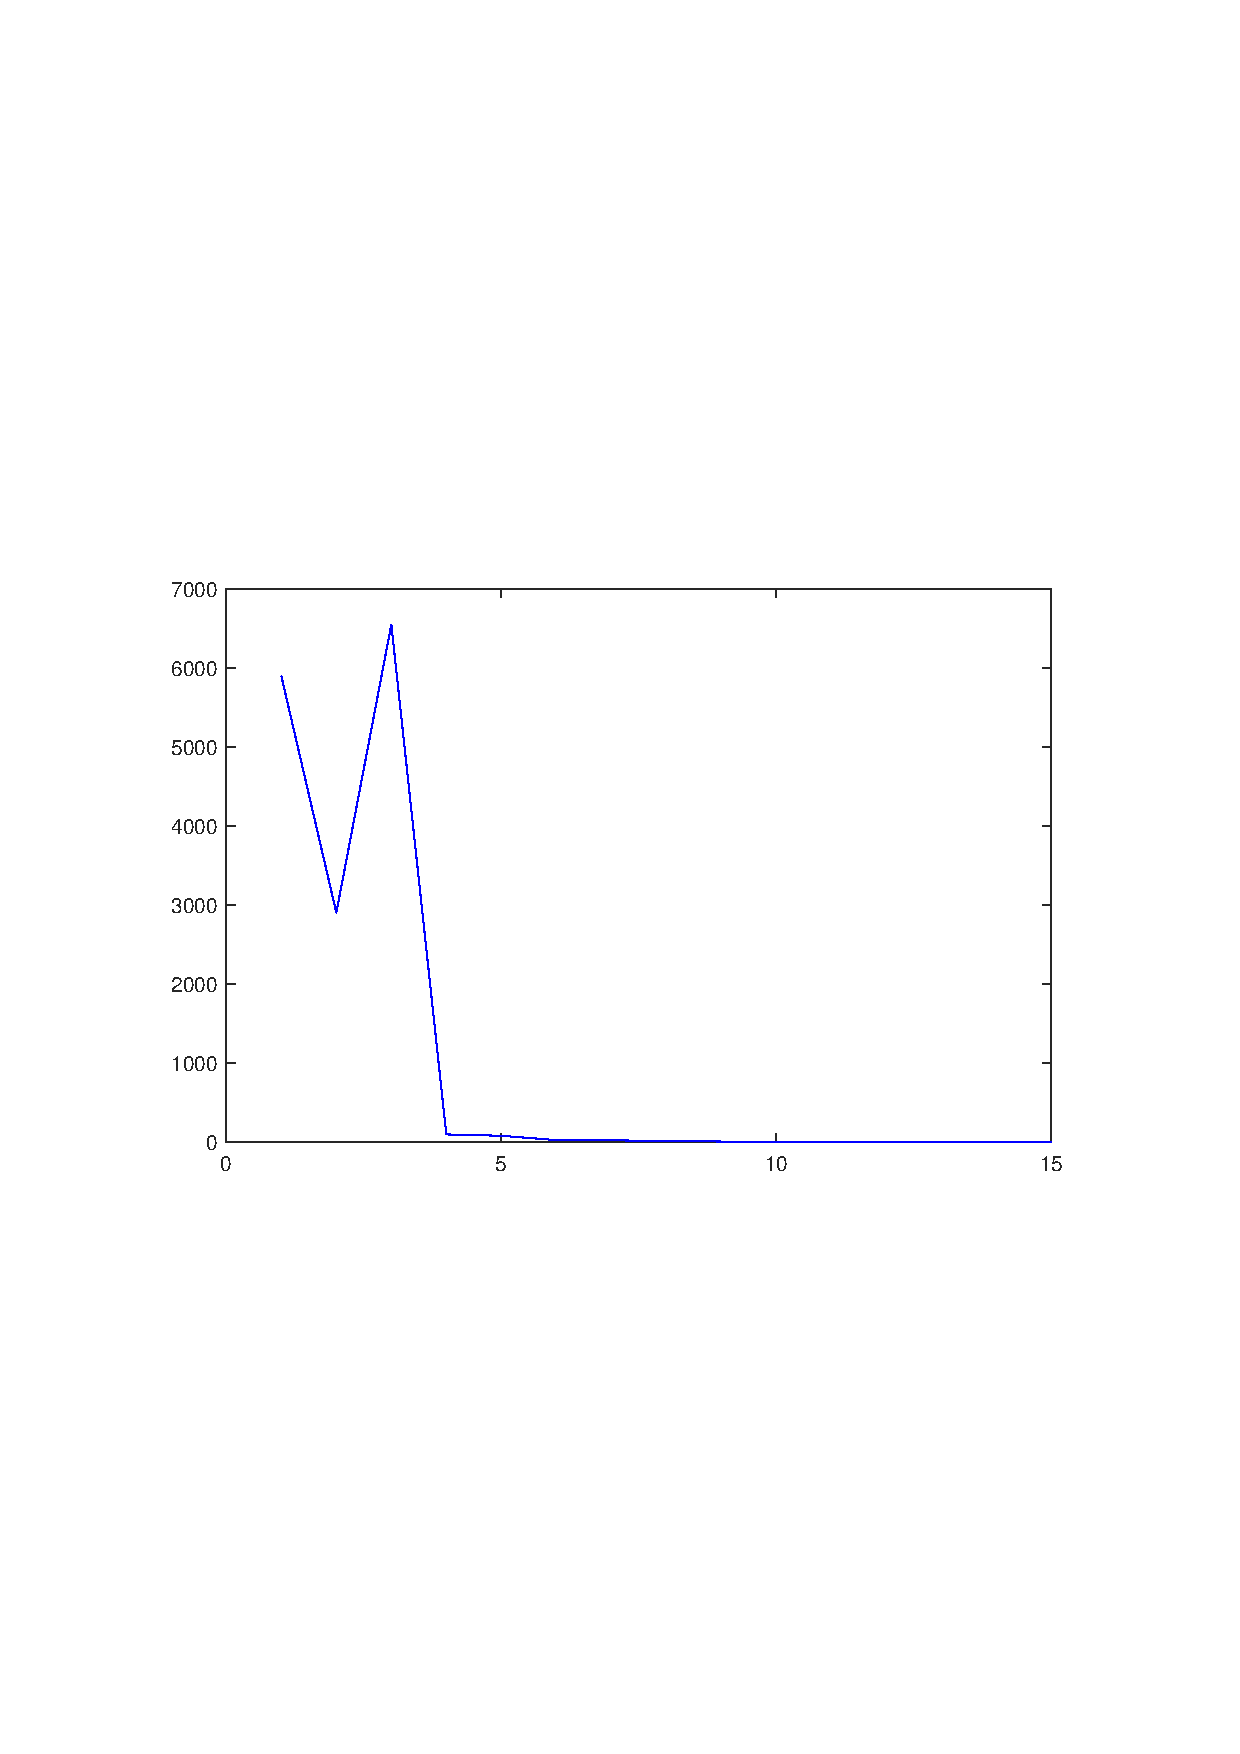
\includegraphics[width=7.5cm]{第二题-BFGS-grad.pdf}\label{BFGS-grad}}
        \caption{BFGS法结果图,$ n=2 $ }
    \end{figure}

    当$ n=3 $时,最终迭代次数为$ 52 $ 次,极小点为$ (-0.37573,0.92779,0.17164) $ ,函数值为$ 0.4714 $ .

    \subsection{上机程序}
    \begin{center}
        \textbf{SR1,DFP,BFGS法上机代码}
    \end{center}

    \lstinputlisting[language=matlab]{SecondAssignment/Newton_Watson.m}

    \renewcommand{\refname}{参考文献}
    \bibliography{reference}
    \bibliographystyle{apacite}
\end{document}